\documentclass[a4paper,11pt]{article}
\usepackage[french]{babel}
\usepackage[T1]{fontenc}

\usepackage{amssymb,amsmath,amsfonts, amsfonts}
\usepackage{enumitem}
\usepackage{multicol}

\usepackage{graphicx}
\usepackage{media9}
\usepackage{listingsutf8}

\newcommand\video[3]{%
\includemedia[%
src=#1,
width=#2,
height=#3,
activate=pageopen
]{}{VPlayer.swf}
}

\newcommand\geogebra[3]{%
\includemedia[%
src=#1,
width=#2,
height=#3,
activate=pageopen
]{}{VPlayer.swf}
}


\begin{document}
\section{Équations du deuxième degré}
\subsection{théorie}
L'expression sous la racine $$\Delta= \mathbf{b^2-4ac}$$ est appelée le \textbf{discriminant} et détermine le nombre de solutions d'une équation quadratique:\\
$\begin{array}{|l | l |}
\hline
\Delta>0 & \text{L'équation a \textbf{deux solutions} réelles} \\
& \text{Le polynôme factorisé est de la forme:}  a(x - x_{1})(x - x_{2}) \\
\hline
\Delta=0 & \text{L'équation a \textbf{une solution} réelle (solution double)}\\
& \text{Le polynôme factorisé est de la forme:}  a(x - x_{1})^2\\
\hline
\Delta<0 & \text{L'équation \textbf{n'a pas de solution} réelle}\\
& \text{Le polynôme ne peut pas être factorisé.}\\
\hline
\end{array}$\par

\subsection{Images}
Du texte avec des images:\par
Soit le triangle rectangle ABC rectangle en C dont $c$ est l'hypoténuse, $a$ et $b$ sont les cathètes et $c_{1}$ et $c_{2}$ sont les segments qui vont du pied de la hauteur ($H$) aux sommets adjacents ($A$ et $B$).\par
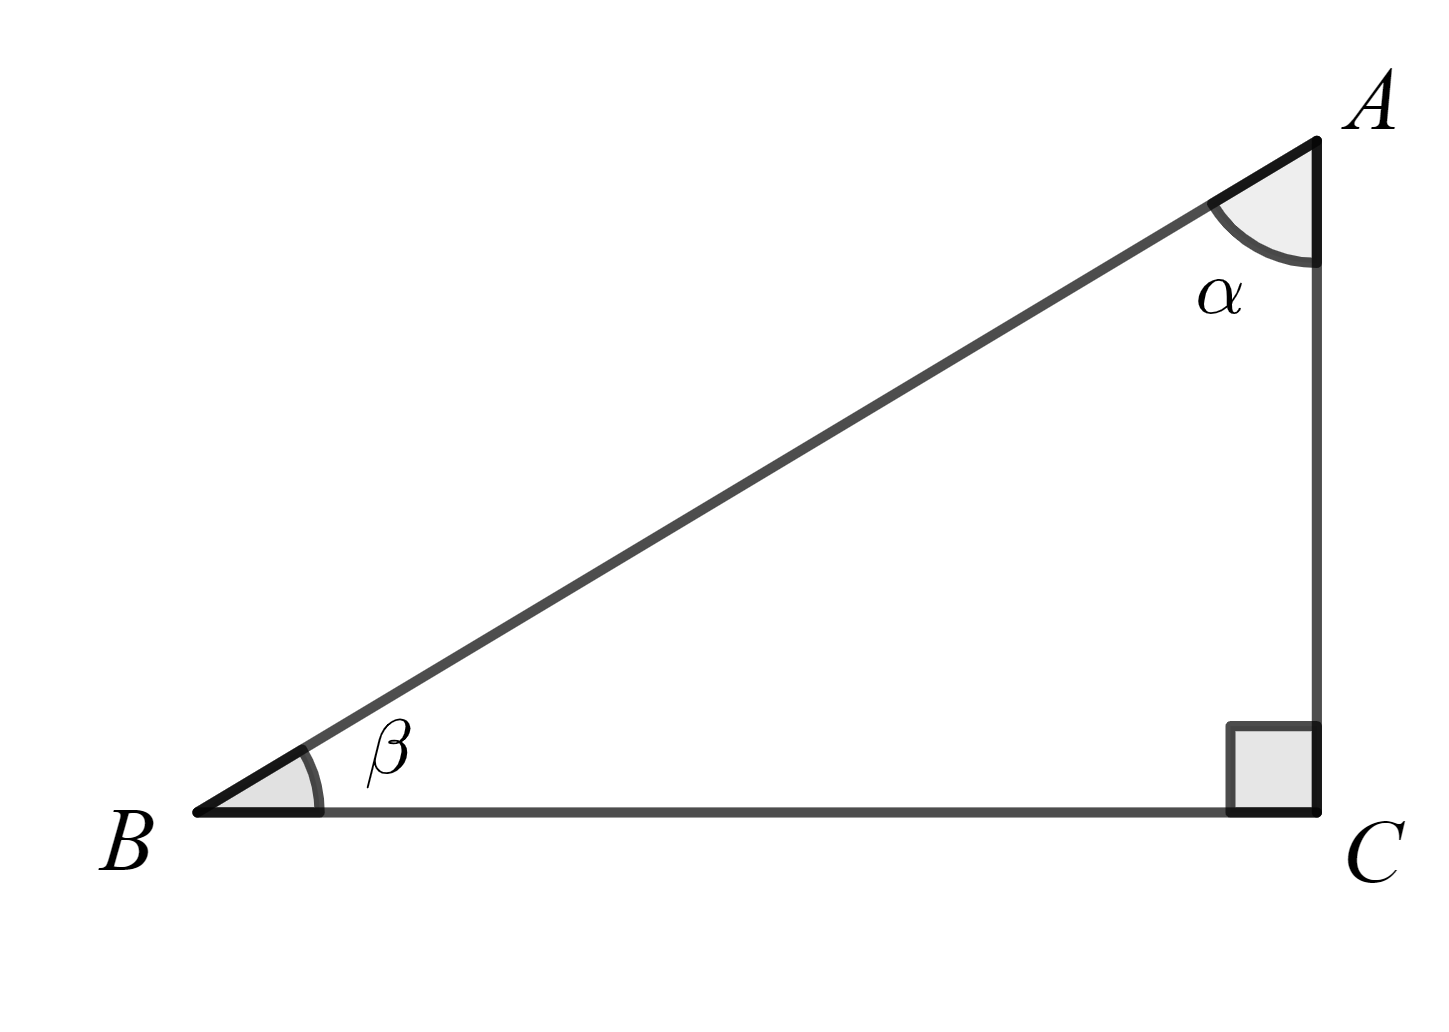
\includegraphics[width=0.5\textwidth]{images/pythagore.png}\\

\subsection{Vidéo}
Ici j'ajoute un lien vers une vidéo youtube:\par
\video{tc9wvbYuZts}{560}{315}

\subsection{Geogebra}
Ici j'ajoute un lien vers un document geogebra:\par
\geogebra{cpmbrfxg}{800}{600}

\subsection{Python}
Ici j'ajoute du code python:\par
% \begin{lstlisting}[language=Python]
% from turtle import *
% from math import sqrt

% def gotoXY(x, y):
%     penup()
%     goto(x, y)
%     pendown()

% def calcul_hypotenuse(cote):
%     return sqrt(2)*cote

% def calcul_cote(hypotenuse):
%     return hypotenuse / sqrt(2)

% def carre(cote, couleur, positionX, positionY, orientation):
%     gotoXY(positionX, positionY)
%     setheading(orientation)
%     fillcolor(couleur)
%     begin_fill()
%     for i in range(4):
%         forward(cote)
%         left(90)
%     end_fill()

% def triangle_iso(cote, couleur, positionX, positionY, orientation):
%     gotoXY(positionX, positionY)
%     setheading(orientation)
%     fillcolor(couleur)
%     begin_fill()
%     forward(cote)
%     left(90)
%     forward(cote)
%     left(180-45)
%     forward(calcul_hypotenuse(cote))
%     end_fill()

% def parallelogramme(cote, couleur, positionX, positionY, orientation):
%     gotoXY(positionX, positionY)
%     setheading(orientation)
%     fillcolor(couleur)
%     begin_fill()
%     for i in range(2):
%         forward(cote)
%         left(45)
%         forward(calcul_hypotenuse(cote))
%         left(135)
%     end_fill()

% speed(0)
% triangle_iso(calcul_cote(800), "blue", -400, -400, 45)
% triangle_iso(calcul_cote(800), "green", -400, 400, -45)
% triangle_iso(calcul_cote(400), "yellow", 0, -400, 135)
% carre(calcul_cote(400), "red", 0, -400, 45)
% triangle_iso(calcul_cote(400), "magenta", 200, 200, -135)
% parallelogramme(calcul_cote(400), "cyan", 200, -200, 45)
% triangle_iso(400, "orange", 0, -400, 0)
% hideturtle()
% \end{lstlisting}

\end{document}
